\subsection{Implementierung und Umsetzung}
\label{subsec:03implementierung}
Die Struktur des Algorithmus der Personenverfolgung mit ihren jeweiligen Modulen ist in Abbildung \ref{fig:personenverfolgung-struktur} dargestellt.
\begin{figure}[btp]
	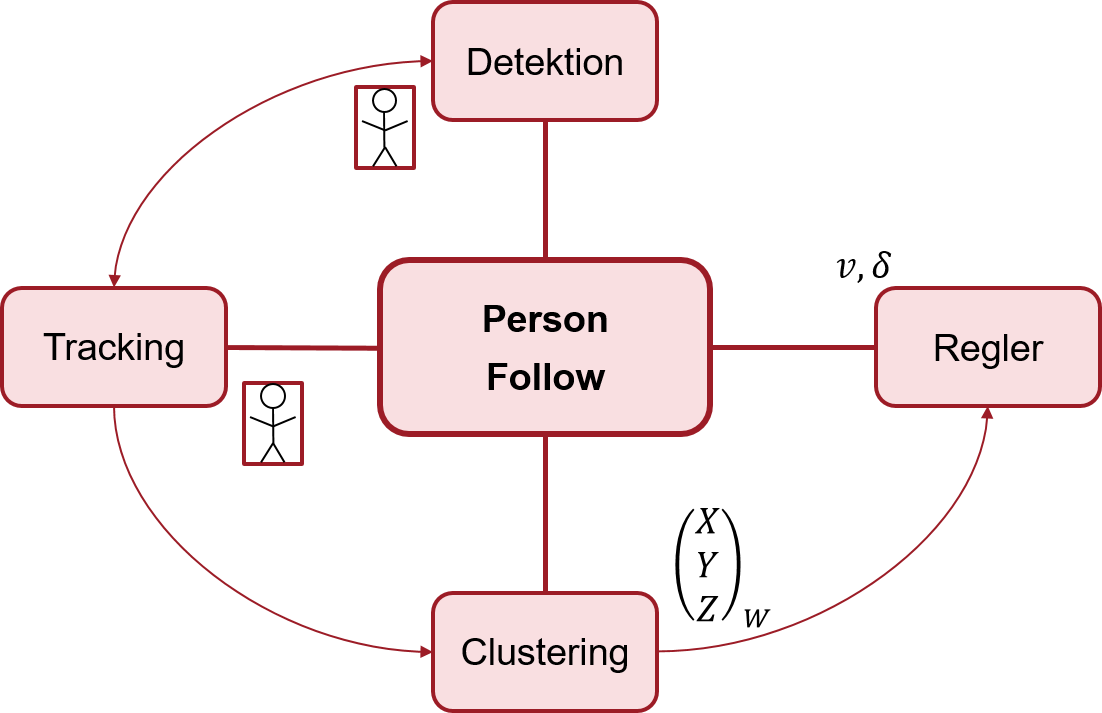
\includegraphics[width=\textwidth]{./pics/personenverfolgung_output.png}
	\caption{Struktur der Personenverfolgung mit jeweiligen Modulen.}
	\label{fig:personenverfolgung-struktur}
\end{figure}
Dabei ist anhand der Pfeilrichtungen gut zu erkennen, wie die einzelnen Module miteinander verkn�pft sind. Anfangs wird mittels der Detektion eine Person im Farbbild detektiert und als Zielperson f�r die Anfahrt festgelegt. Letzteres wird umgesetzt, indem eine Bounding Box der Person erstellt wird. Da diese Detektion stetig stattfindet, ist sie ziemlich rechenaufw�ndig. Die Bildrate der Kamera des Autos f�llt dabei stark ab. Daher ist die Kombination mit einem Tracker notwendig. Dieser wird aktiviert, sobald eine Personendetektion erfolgt und bekommt die entsprechende Bounding Box �bergeben. Da Trackeralgorithmen grunds�tzlich mit einem gewissen Drift der Position der Person bzw. des Objektes einhergehen ist eine Umschaltung zur Detektion nach einer gewissen Zeit sinnvoll, um die Korrektheit der Bounding Box wiederherzustellen. Somit findet ein stetiger Wechsel beider Module statt. Im Modul Clustering findet die Berechnung der Personenkoordinaten statt. Dazu wird die Bounding Box des Farbbildes auf das Tiefenbild projiziert. Innerhalb der Bounding Box des Tiefenbildes wird die Person von der Umgebung extrahiert und ihre Tiefe bestimmt. Mithilfe dieser und der Projektionsmatrix werden die Koordinaten der Person berechnet. Diese bekommt der Regler �bergeben, welcher daraus das finale Ziel berechnet und einen entsprechenden Lenkwinkel $\theta$ und eine entsprechende Geschwindigkeit $v$ vorgibt.